\chapter{Implementation}\label{chapter:implementation}

This project has been implemented as an MITK plugin. MITK, the Medical Imaging Interaction Toolkit, is a free open-source software system for the development of interactive medical image processing software. It combines ITK (for image processing) and VTK (for visualization) together with a basic application, the MITK Workbench, that can be extended with plugins. The UI for the plugin is based on Qt.

\begin{figure}[H]
  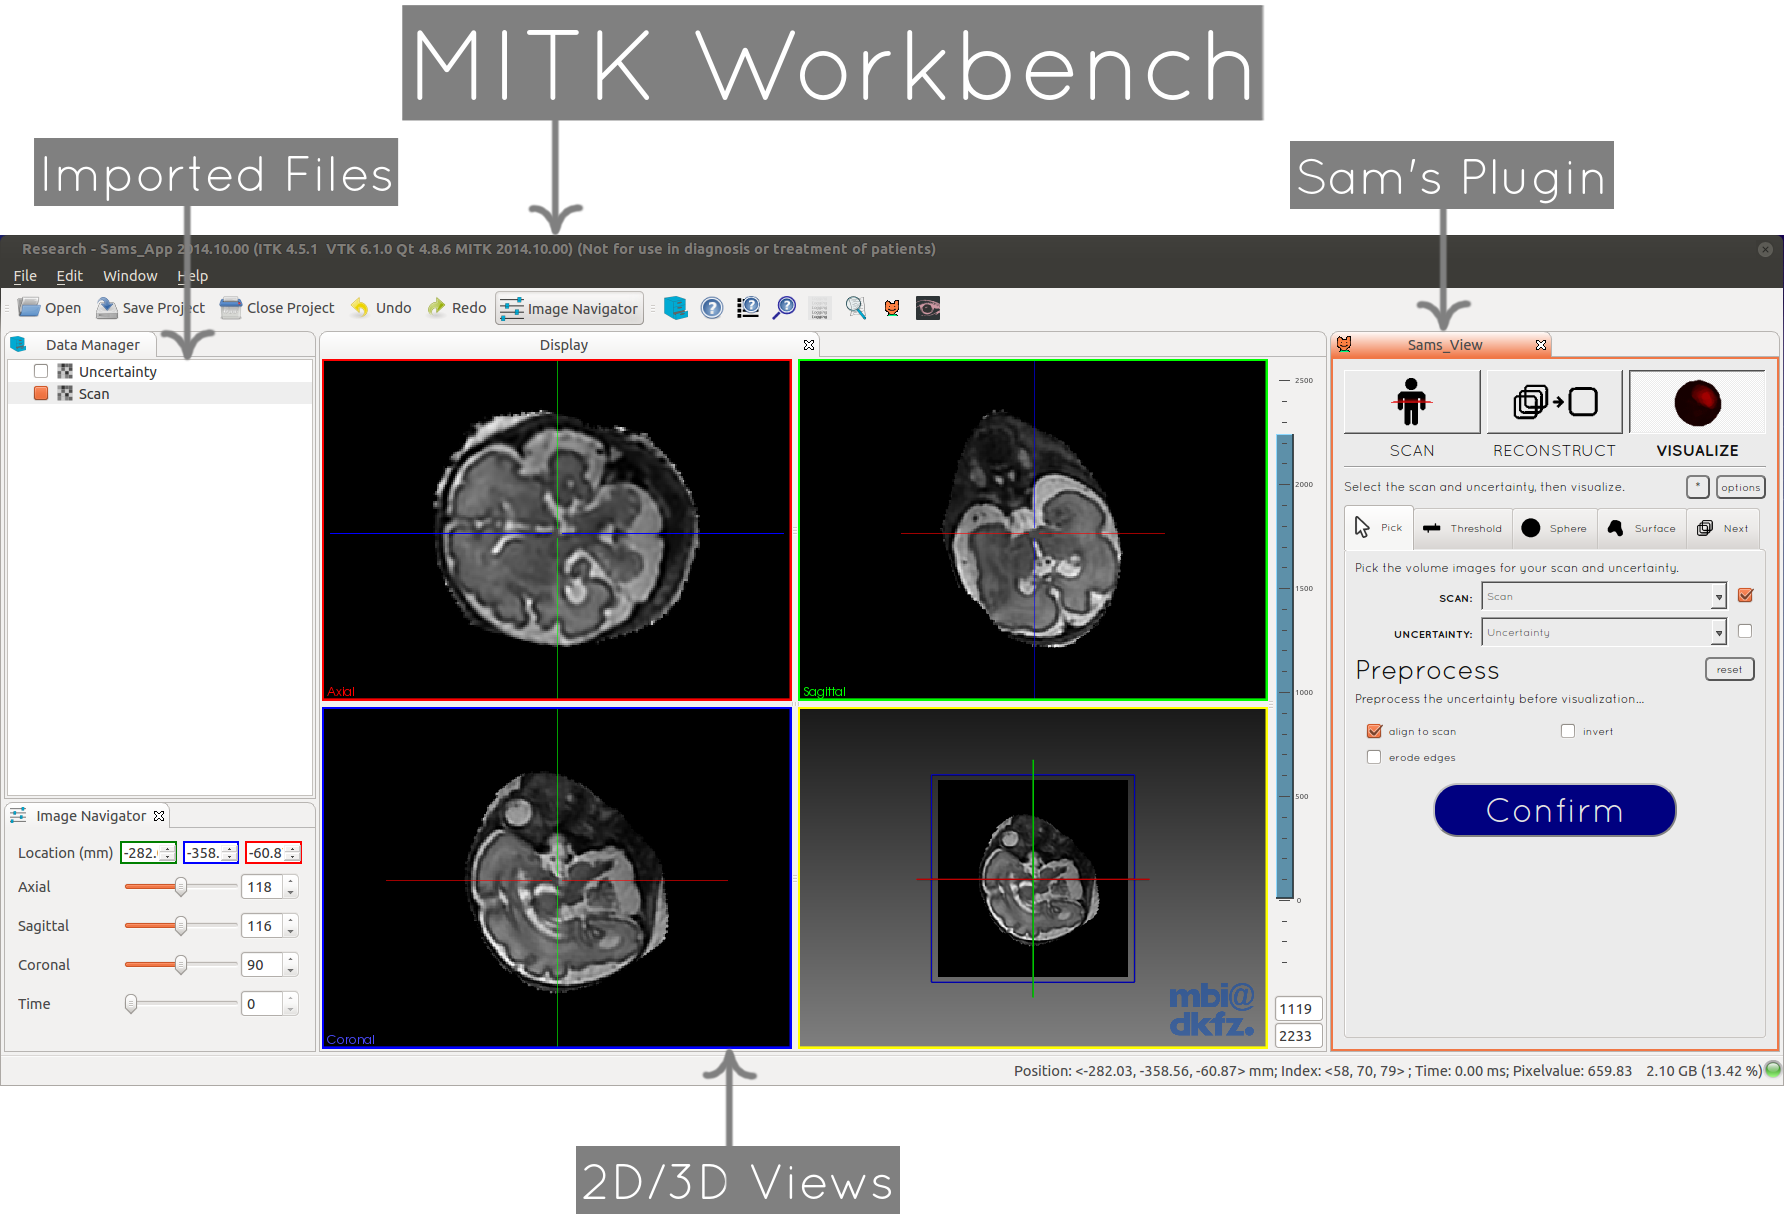
\includegraphics[width=\textwidth]{images/tool/mitk.png}
  \caption{MITK Workbench + Plugin}\label{fig:mitkoverview}
\end{figure}

The plugin developed is a research prototype designed primarily to visualize the uncertainty in MRI reconstructions. It also begins to integrate all parts of the reconstruction pipeline together in one application. Broadly speaking the pipeline can be split into three steps: scan -> reconstruct -> visualize. 

Components from each stage have been incorporated into the plugin. Firstly a scan can be simulated by taking a previous reconstruction and resampling it. Then scans, simulated or otherwise, can be used to reconstruct a super-resolution image and optionally landmarks can be provided to guide this process. Finally the reconstructed volume, and associated uncertainty, can be visualized and the next best scan plane can be determined. The rest of this chapter shows the implementation of all of these features.

\section{Scan Simulation}\label{implementation:simulatescan}
The idea behind simulating a scan is that we can evaluate the performance of reconstruction algorithms if we can compare the result to a known, 'perfect', reconstruction. This idea was used in the same paper concerned with finding the optimum scan plane\cite{uncertaintysvd}. The focus of this part of the tool is not to evaluate the effectiveness of this approach, that is a project in it's own right, but to make this simulation easier to perform and customize for future research.

\begin{wrapfigure}[23]{r}{0.4\textwidth}
  \vspace{-20pt}
  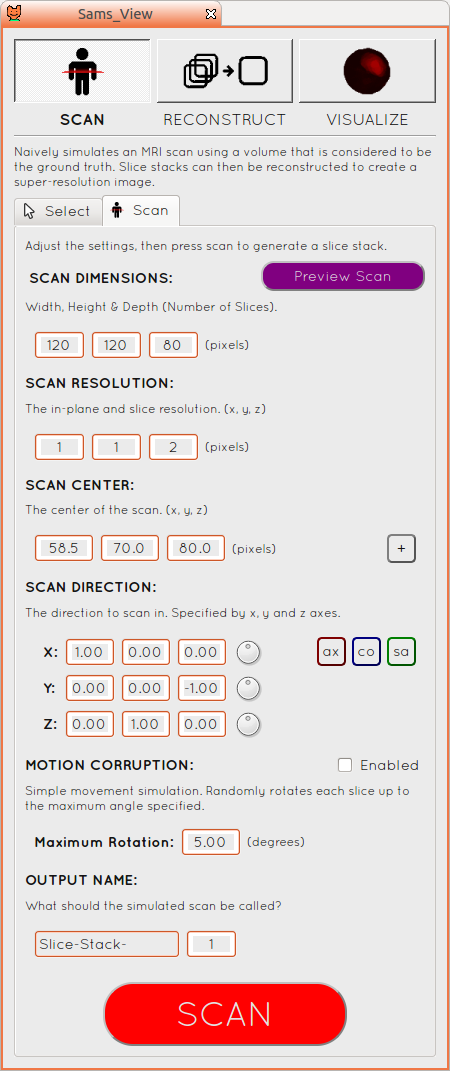
\includegraphics[width=0.4\textwidth]{images/scan_simulation/scan_settings.png}
  \caption{Controls}\label{fig:scansettings}
\end{wrapfigure}

The user has a number of controls (see figure \ref{fig:scansettings}) available to tweak:

\subsection*{Scan Dimensions}
Number of pixels in the scan (x, y, z).

\subsection*{Scan Resolution}
Size of each pixel, relative to the reconstructed scan (x, y, z).

\subsection*{Scan Center}
The center point of the scan (x, y, z). This can be set to the center of the volume or adjusted manually.

\subsection*{Scan Direction}
The direction to scan in. You may expect this to be just one vector (the z-direction) but since the scan is rectangular in shape the x and y-direction also need to be specified. The standard axial, coronal and sagittal directions are available and the direction can be rotated about each axis using the dials.

\subsection*{Motion Corruption}
Some simple motion corruption can be enabled. Currently the implementation is quite simple; the motion only happens in between slices being scanned. Before each slice gets scanned a random rotation (up to a maximum specified) is applied about a random axis to the original image.

A preview to illustrate the area that the scan configured is overlayed on the volume. Whenever any control changes this preview updates. Figure \ref{fig:scansimulationexample} shows an example of an axial scan (y-axis) simulated with 5 degrees of motion corruption. Note that when viewed from the side adjacent stacks don't line up.

\begin{figure}[H]
  \centering
  \begin{subfigure}[b]{0.5\textwidth}
    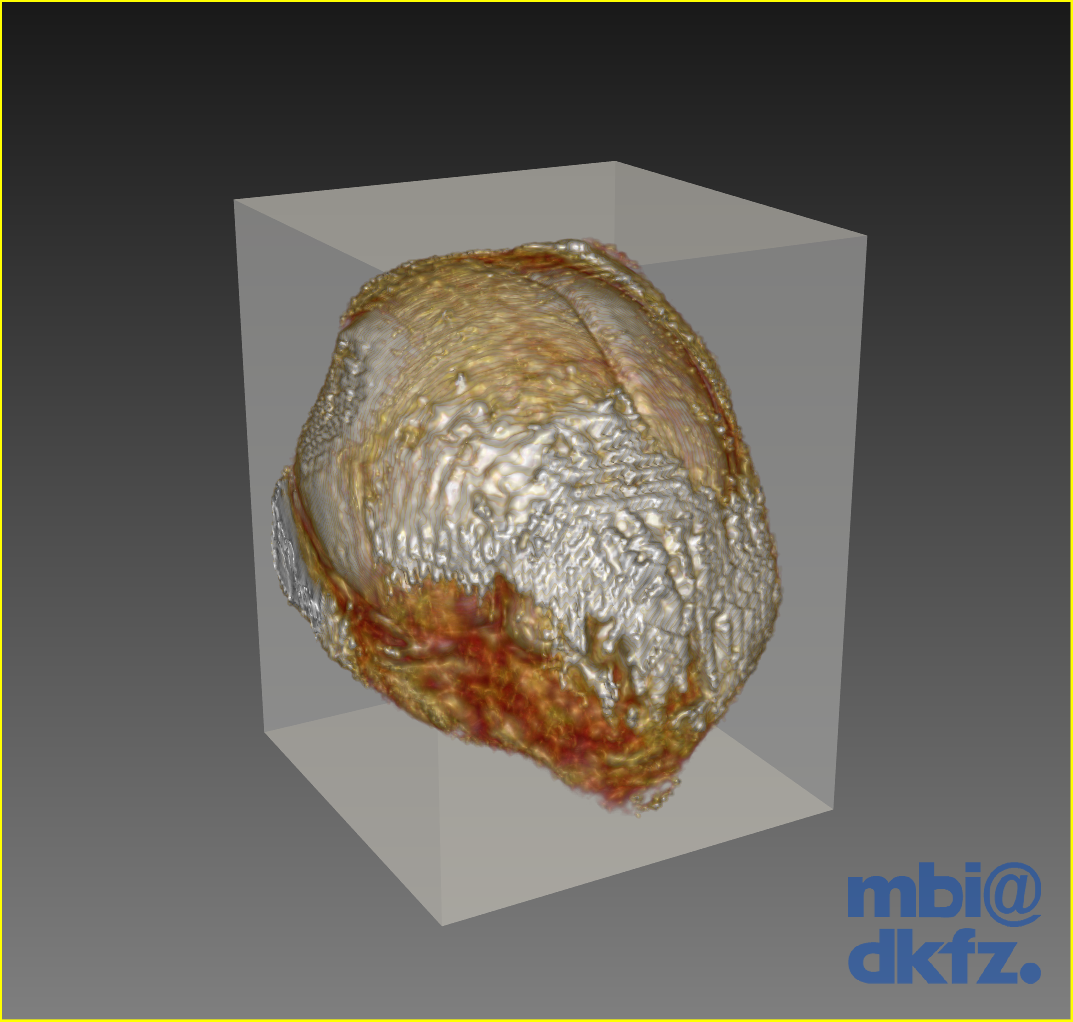
\includegraphics[width=\textwidth]{images/scan_simulation/scan_axial_preview.png}
    \caption{Scan Preview}\label{fig:scansimulationpreview}
  \end{subfigure}%
  ~ %add desired spacing between images, e. g. ~, \quad, \qquad, \hfill etc.
    %(or a blank line to force the subfigure onto a new line)
  \begin{subfigure}[b]{0.5\textwidth}
    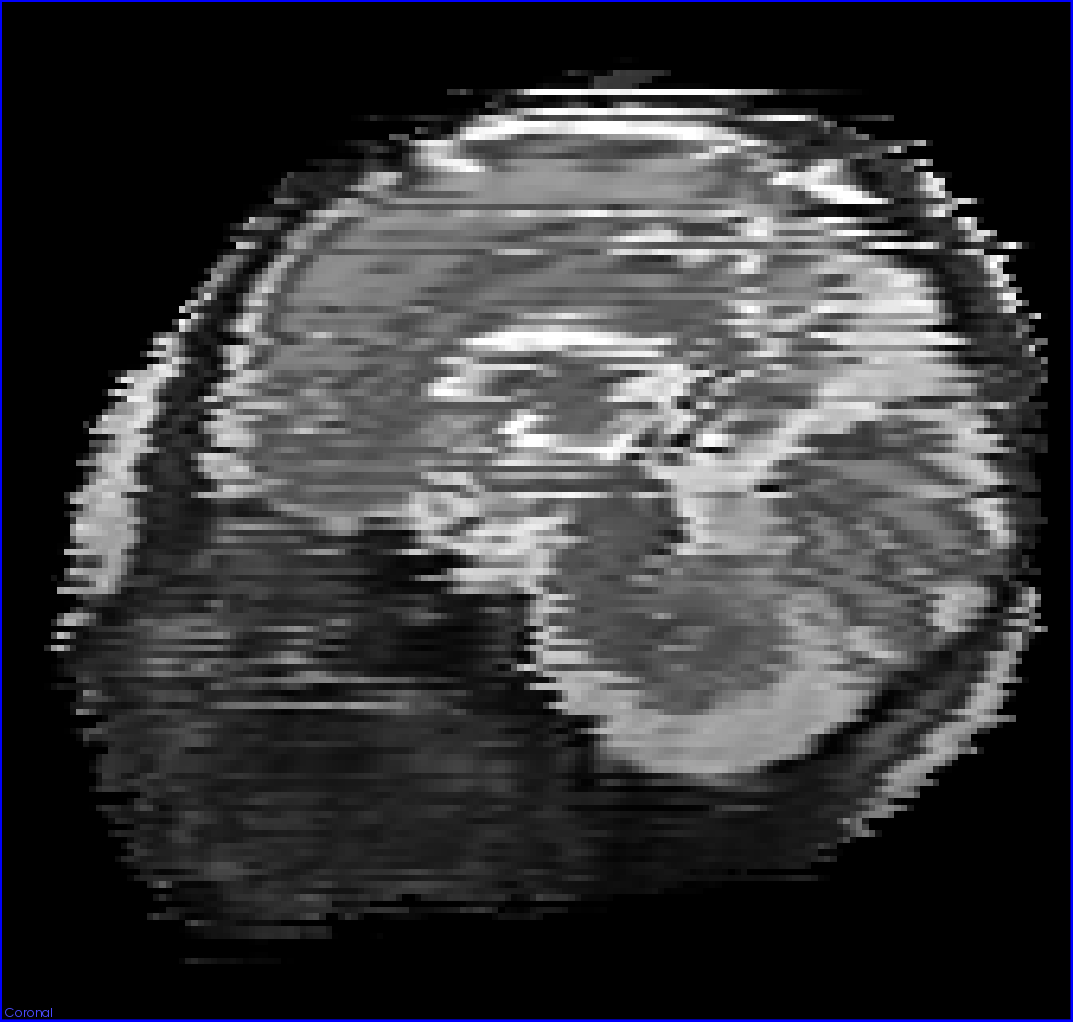
\includegraphics[width=\textwidth]{images/scan_simulation/scan_axial_result.png}
    \caption{Side (Sagittal) View of Simulation}\label{fig:scansimulationresult}
  \end{subfigure}
  \caption{Example Scan Simulation}\label{fig:scansimulationexample}
\end{figure}

\clearpage
\section{Reconstruction}\label{implementation:reconstruction}
Screenshot. Explain controls.

\clearpage
\section{Visualizations}\label{implementation:visualizations}

\subsection{Thresholding}\label{implementation:thresholding}
Screenshot. Explain controls.

\subsection{Sphere}\label{implementation:sphere}
Screenshot. Explain controls.

\subsection{Surface}\label{implementation:surface}
Screenshot. Explain controls.

\subsection{Next Scan Plane}\label{implementation:nextscanplane}
Screenshot. Explain controls.